\documentclass[]{article}
\usepackage{lmodern}
\usepackage{amssymb,amsmath}
\usepackage{ifxetex,ifluatex}
\usepackage{fixltx2e} % provides \textsubscript
\ifnum 0\ifxetex 1\fi\ifluatex 1\fi=0 % if pdftex
  \usepackage[T1]{fontenc}
  \usepackage[utf8]{inputenc}
\else % if luatex or xelatex
  \ifxetex
    \usepackage{mathspec}
  \else
    \usepackage{fontspec}
  \fi
  \defaultfontfeatures{Ligatures=TeX,Scale=MatchLowercase}
\fi
% use upquote if available, for straight quotes in verbatim environments
\IfFileExists{upquote.sty}{\usepackage{upquote}}{}
% use microtype if available
\IfFileExists{microtype.sty}{%
\usepackage{microtype}
\UseMicrotypeSet[protrusion]{basicmath} % disable protrusion for tt fonts
}{}
\usepackage[margin=1in]{geometry}
\usepackage{hyperref}
\hypersetup{unicode=true,
            pdftitle={Lista 5 - MAE0514},
            pdfauthor={Guilherme NºUSP: 8943160 e Leonardo NºUSP: 9793436},
            pdfborder={0 0 0},
            breaklinks=true}
\urlstyle{same}  % don't use monospace font for urls
\usepackage{color}
\usepackage{fancyvrb}
\newcommand{\VerbBar}{|}
\newcommand{\VERB}{\Verb[commandchars=\\\{\}]}
\DefineVerbatimEnvironment{Highlighting}{Verbatim}{commandchars=\\\{\}}
% Add ',fontsize=\small' for more characters per line
\usepackage{framed}
\definecolor{shadecolor}{RGB}{248,248,248}
\newenvironment{Shaded}{\begin{snugshade}}{\end{snugshade}}
\newcommand{\KeywordTok}[1]{\textcolor[rgb]{0.13,0.29,0.53}{\textbf{#1}}}
\newcommand{\DataTypeTok}[1]{\textcolor[rgb]{0.13,0.29,0.53}{#1}}
\newcommand{\DecValTok}[1]{\textcolor[rgb]{0.00,0.00,0.81}{#1}}
\newcommand{\BaseNTok}[1]{\textcolor[rgb]{0.00,0.00,0.81}{#1}}
\newcommand{\FloatTok}[1]{\textcolor[rgb]{0.00,0.00,0.81}{#1}}
\newcommand{\ConstantTok}[1]{\textcolor[rgb]{0.00,0.00,0.00}{#1}}
\newcommand{\CharTok}[1]{\textcolor[rgb]{0.31,0.60,0.02}{#1}}
\newcommand{\SpecialCharTok}[1]{\textcolor[rgb]{0.00,0.00,0.00}{#1}}
\newcommand{\StringTok}[1]{\textcolor[rgb]{0.31,0.60,0.02}{#1}}
\newcommand{\VerbatimStringTok}[1]{\textcolor[rgb]{0.31,0.60,0.02}{#1}}
\newcommand{\SpecialStringTok}[1]{\textcolor[rgb]{0.31,0.60,0.02}{#1}}
\newcommand{\ImportTok}[1]{#1}
\newcommand{\CommentTok}[1]{\textcolor[rgb]{0.56,0.35,0.01}{\textit{#1}}}
\newcommand{\DocumentationTok}[1]{\textcolor[rgb]{0.56,0.35,0.01}{\textbf{\textit{#1}}}}
\newcommand{\AnnotationTok}[1]{\textcolor[rgb]{0.56,0.35,0.01}{\textbf{\textit{#1}}}}
\newcommand{\CommentVarTok}[1]{\textcolor[rgb]{0.56,0.35,0.01}{\textbf{\textit{#1}}}}
\newcommand{\OtherTok}[1]{\textcolor[rgb]{0.56,0.35,0.01}{#1}}
\newcommand{\FunctionTok}[1]{\textcolor[rgb]{0.00,0.00,0.00}{#1}}
\newcommand{\VariableTok}[1]{\textcolor[rgb]{0.00,0.00,0.00}{#1}}
\newcommand{\ControlFlowTok}[1]{\textcolor[rgb]{0.13,0.29,0.53}{\textbf{#1}}}
\newcommand{\OperatorTok}[1]{\textcolor[rgb]{0.81,0.36,0.00}{\textbf{#1}}}
\newcommand{\BuiltInTok}[1]{#1}
\newcommand{\ExtensionTok}[1]{#1}
\newcommand{\PreprocessorTok}[1]{\textcolor[rgb]{0.56,0.35,0.01}{\textit{#1}}}
\newcommand{\AttributeTok}[1]{\textcolor[rgb]{0.77,0.63,0.00}{#1}}
\newcommand{\RegionMarkerTok}[1]{#1}
\newcommand{\InformationTok}[1]{\textcolor[rgb]{0.56,0.35,0.01}{\textbf{\textit{#1}}}}
\newcommand{\WarningTok}[1]{\textcolor[rgb]{0.56,0.35,0.01}{\textbf{\textit{#1}}}}
\newcommand{\AlertTok}[1]{\textcolor[rgb]{0.94,0.16,0.16}{#1}}
\newcommand{\ErrorTok}[1]{\textcolor[rgb]{0.64,0.00,0.00}{\textbf{#1}}}
\newcommand{\NormalTok}[1]{#1}
\usepackage{longtable,booktabs}
\usepackage{graphicx,grffile}
\makeatletter
\def\maxwidth{\ifdim\Gin@nat@width>\linewidth\linewidth\else\Gin@nat@width\fi}
\def\maxheight{\ifdim\Gin@nat@height>\textheight\textheight\else\Gin@nat@height\fi}
\makeatother
% Scale images if necessary, so that they will not overflow the page
% margins by default, and it is still possible to overwrite the defaults
% using explicit options in \includegraphics[width, height, ...]{}
\setkeys{Gin}{width=\maxwidth,height=\maxheight,keepaspectratio}
\IfFileExists{parskip.sty}{%
\usepackage{parskip}
}{% else
\setlength{\parindent}{0pt}
\setlength{\parskip}{6pt plus 2pt minus 1pt}
}
\setlength{\emergencystretch}{3em}  % prevent overfull lines
\providecommand{\tightlist}{%
  \setlength{\itemsep}{0pt}\setlength{\parskip}{0pt}}
\setcounter{secnumdepth}{0}
% Redefines (sub)paragraphs to behave more like sections
\ifx\paragraph\undefined\else
\let\oldparagraph\paragraph
\renewcommand{\paragraph}[1]{\oldparagraph{#1}\mbox{}}
\fi
\ifx\subparagraph\undefined\else
\let\oldsubparagraph\subparagraph
\renewcommand{\subparagraph}[1]{\oldsubparagraph{#1}\mbox{}}
\fi

%%% Use protect on footnotes to avoid problems with footnotes in titles
\let\rmarkdownfootnote\footnote%
\def\footnote{\protect\rmarkdownfootnote}

%%% Change title format to be more compact
\usepackage{titling}

% Create subtitle command for use in maketitle
\providecommand{\subtitle}[1]{
  \posttitle{
    \begin{center}\large#1\end{center}
    }
}

\setlength{\droptitle}{-2em}

  \title{Lista 5 - MAE0514}
    \pretitle{\vspace{\droptitle}\centering\huge}
  \posttitle{\par}
    \author{Guilherme NºUSP: 8943160 e Leonardo NºUSP: 9793436}
    \preauthor{\centering\large\emph}
  \postauthor{\par}
    \date{}
    \predate{}\postdate{}
  
\usepackage{multirow}
\usepackage{ragged2e}

\begin{document}
\maketitle

\section{Exercício 1}\label{exercicio-1}

Considere o conjunto de dados de pacientes com leucemia aguda que
receberam transplante de medula óssea, apresentado na seção 1.3 de Klein
e Moeschberger (2003). Os pacientes que recebem transplante de doador
compatível (alogênico) podem desenvolver uma doença conhecida como DECH
(doença do enxerto contra o hospedeiro) ou GVHD (graft-versus-host
disease), que pode ser muito grave. No entanto, suspeita-se que DECH
tenha um efeito anti-leucêmico nos pacientes. Para verificar essa
hipótese, deseja-se ajustar um modelo de Cox aos dados, considerando-se
como variável resposta o tempo até a recorrência da doença (relapse).
Pacientes que apresentaram óbito antes da recorrência são considerados
como observações censuradas. Os dados que devem ser utilizados estão
disponíveis no arquivo BMT-Data.csv e a descrição das variáveis está no
arquivo BMT-Data.des.

\begin{enumerate}
\def\labelenumi{(\alph{enumi})}
\tightlist
\item
  Defina duas variáveis dependentes do tempo indicadoras da ocorrência
  de DECH aguda e crônica. Escreva o modelo semiparamétrico de Cox
  incluindo as variáveis idade do paciente, sexo do paciente, tempo até
  o transplante, classificação morfológica Franco-AmericanaBritâneica
  (FAB) e tratamento profilático para DECH (MTX), além das variáveis
  dependentes do tempo definidas.
\end{enumerate}

\subsection{Resolução}\label{resolucao}

Inicialmente defindo as duas variáveis dependentes do tempo indicadoras
da ocorrência de DECH aguda e crônica que no banco de dados são ``A'' e
``C'' respectivamente, sendo ambas covariáveis do tipo internas, ou
seja, são medidas no indivíduo quando o paciente estava em observação,
em relação o tempo até a recorrência da doença.

O modelo semi-paramétrico de cox pode ser escrito como:

\[\alpha(t|x(t))=\alpha_0(t)e^{x'(t)\beta}\]

Em que \(\alpha(t|x(t))\) é a função de taxa de falha a ser modelada, a
matriz \(x(t)\) é conhecida para todo instante no qual a observação
``i'' está sendo acompanhada (ao longo do tempo), \(\alpha_0(t)\) é a
função de taxa de falha de referência e por fim \(\beta\) é o vetor de
parâmetros do modelo.

\begin{enumerate}
\def\labelenumi{(\alph{enumi})}
\setcounter{enumi}{1}
\tightlist
\item
  Ajuste um modelo de Cox com as variáveis do item (a). Selecione as
  variáveis significativas e faça a verificação da proporcionalidade dos
  riscos. O que pode ser concluído?
\end{enumerate}

\subsection{Resolução}\label{resolucao-1}

Fazendo o ajuste do banco de dados para o formato ``longo'' e ajustando
o modelo com as covariáveis idade do paciente (Z1), sexo do paciente
(Z3), tempo até o transplante (Z7), classificação morfológica
Franco-Americana Britâneica (Z8) e tratamento profilático para DECH
(Z10) e as covariáveis indicadoras da ocorrência de DECH aguda (A) e
crônica (C) e com isso temos:

\begin{verbatim}
## Call:
## coxph(formula = Surv(Tinicio, Tfim, Delta2) ~ A + C + Z1 + Z3 + 
##     Z7 + Z8 + Z10, data = BMT_DataRELAPSED)
## 
##   n= 223, number of events= 43 
## 
##           coef  exp(coef)   se(coef)      z Pr(>|z|)   
## A   -0.4753906  0.6216422  0.4856246 -0.979  0.32762   
## C    0.2505825  1.2847736  0.3869404  0.648  0.51724   
## Z1   0.0004414  1.0004415  0.0180202  0.024  0.98046   
## Z3  -0.2633559  0.7684684  0.3172550 -0.830  0.40648   
## Z7  -0.0003670  0.9996330  0.0006393 -0.574  0.56587   
## Z8   0.9989454  2.7154166  0.3131941  3.190  0.00142 **
## Z10  0.4787014  1.6139772  0.3460418  1.383  0.16655   
## ---
## Signif. codes:  0 '***' 0.001 '**' 0.01 '*' 0.05 '.' 0.1 ' ' 1
## 
##     exp(coef) exp(-coef) lower .95 upper .95
## A      0.6216     1.6086    0.2400     1.610
## C      1.2848     0.7783    0.6018     2.743
## Z1     1.0004     0.9996    0.9657     1.036
## Z3     0.7685     1.3013    0.4126     1.431
## Z7     0.9996     1.0004    0.9984     1.001
## Z8     2.7154     0.3683    1.4698     5.017
## Z10    1.6140     0.6196    0.8191     3.180
## 
## Concordance= 0.689  (se = 0.037 )
## Likelihood ratio test= 14.94  on 7 df,   p=0.04
## Wald test            = 14.81  on 7 df,   p=0.04
## Score (logrank) test = 15.95  on 7 df,   p=0.03
\end{verbatim}

Agora fazendo a verificação das variáveis mais significativas, temos:

\begin{longtable}[]{@{}lrrrr@{}}
\toprule
& Df & AIC & LRT & Pr(\textgreater{}Chi)\tabularnewline
\midrule
\endhead
& NA & 389.034 & NA & NA\tabularnewline
A & 1 & 388.103 & 1.070 & 0.301\tabularnewline
C & 1 & 387.450 & 0.416 & 0.519\tabularnewline
Z1 & 1 & 387.034 & 0.001 & 0.980\tabularnewline
Z3 & 1 & 387.721 & 0.687 & 0.407\tabularnewline
Z7 & 1 & 387.407 & 0.373 & 0.541\tabularnewline
Z8 & 1 & 396.955 & 9.921 & 0.002\tabularnewline
Z10 & 1 & 388.858 & 1.824 & 0.177\tabularnewline
\bottomrule
\end{longtable}

Em que apenas a variável ``Z8'' que corresponde a classificação
morfológica Franco-Americana Britâneica (FAB) é significante, assim
ajustando o modelo novamente obtemos o seguinte resultado:

\begin{verbatim}
## Call:
## coxph(formula = Surv(Tinicio, Tfim, Delta2) ~ Z8, data = BMT_DataRELAPSED)
## 
##   n= 223, number of events= 43 
## 
##      coef exp(coef) se(coef)     z Pr(>|z|)   
## Z8 0.9865    2.6818   0.3059 3.225  0.00126 **
## ---
## Signif. codes:  0 '***' 0.001 '**' 0.01 '*' 0.05 '.' 0.1 ' ' 1
## 
##    exp(coef) exp(-coef) lower .95 upper .95
## Z8     2.682     0.3729     1.473     4.884
## 
## Concordance= 0.618  (se = 0.038 )
## Likelihood ratio test= 10.08  on 1 df,   p=0.001
## Wald test            = 10.4  on 1 df,   p=0.001
## Score (logrank) test = 11.26  on 1 df,   p=8e-04
\end{verbatim}

Resísudos de Schoenfeld:

\begin{center}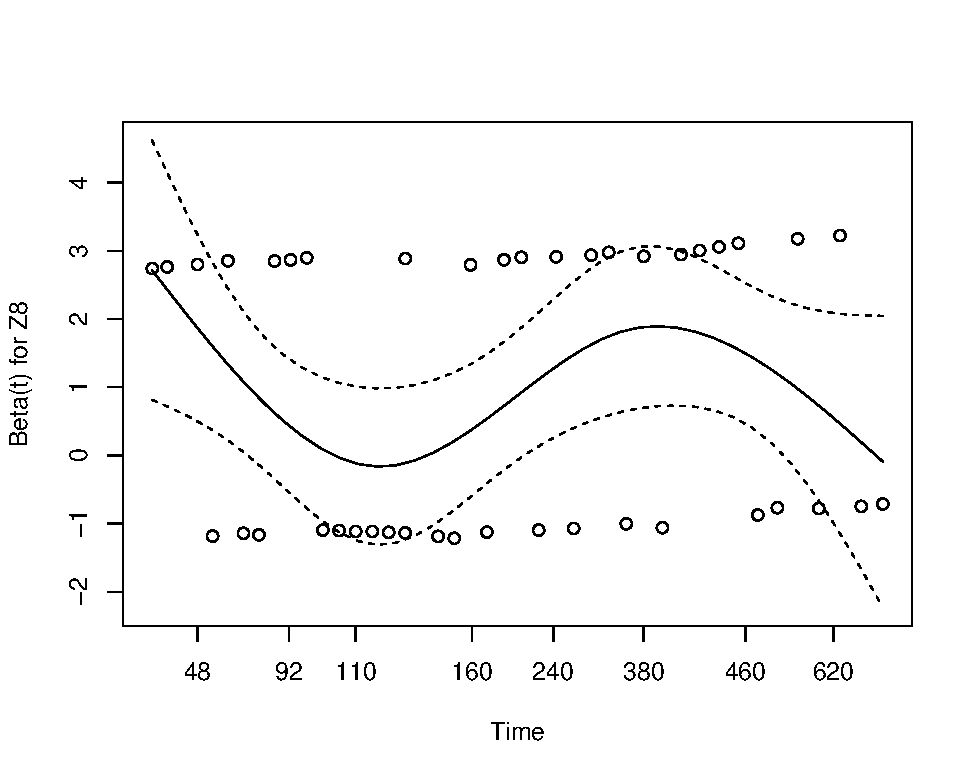
\includegraphics[width=0.8\linewidth]{Lista_5_files/figure-latex/unnamed-chunk-4-1} \end{center}

Em que se pode notar que a variável tratamento apresenta um
comportamento próximo de linear, não sendo possível traçar uma reta ao
longo do tempo.

Fazendo a tabela com o resultado do teste, em que:
\[ \left\{ \begin{array}{ll}
H_0: O \ modelo \ e \ de \ riscos \ proporcionais \\
H_1: O \ modelo \ nao \ e \ de \ riscos \ proporcionais  \end{array} \right.\ \]

\begin{longtable}[]{@{}lrrr@{}}
\toprule
& chisq & df & p\tabularnewline
\midrule
\endhead
Z8 & 0.009 & 1 & 0.925\tabularnewline
GLOBAL & 0.009 & 1 & 0.925\tabularnewline
\bottomrule
\end{longtable}

Queremos testar se o modelo de riscos proporcionais se adequa a esse
caso, e ao observar a tabela acima assim como resultado do gráfico acima
a variável tratamento não se rejeita a hipótese nula com um p-valor de
0.925 considerando um nível de significância de 5\%, ou seja, ela se
adequa no modelo de riscos proporcionais.

E com isso podemos concluir que as funções de sobrevivência para
indivíduos com a variável Z8 igual a 0 e igual a 1 são razoavelmente
paralelas ao longo de todo tempo. Ainda é possível dizer que indivíduos
que assumem o valor 1 para a variável Z8 possuem 2.682 vezes de ter
recorrência da doença (relapse) em relação a indivíduos que assumem o
valor 0 para a variável Z8.

\begin{enumerate}
\def\labelenumi{(\alph{enumi})}
\setcounter{enumi}{2}
\tightlist
\item
  Repita os itens (a) e (b) utilizando o tempo até o óbito como variável
  reposta.
\end{enumerate}

\subsection{Resolução}\label{resolucao-2}

\begin{enumerate}
\def\labelenumi{\alph{enumi})}
\tightlist
\item
  Defindo as duas variáveis dependentes do tempo indicadoras da
  ocorrência de DECH aguda e crônica que no banco de dados são ``A'' e
  ``C'' respectivamente, sendo ambas covariáveis do tipo externa, ou
  seja, podem influenciar no risco de falha, mas não dependem do
  processo de falha, em relação ao tempo até o óbito
\end{enumerate}

O modelo semi-paramétrico de cox pode ser escrito como:

\[\alpha(t|x(t))=\alpha_0(t)e^{x'(t)\beta}\]

Em que \(\alpha(t|x(t))\) é a função de taxa de falha a ser modelada, a
matriz \(x(t)\) é conhecida para todo instante no qual a observação
``i'' está sendo acompanhada (ao longo do tempo), \(\alpha_0(t)\) é a
função de taxa de falha de referência e por fim \(\beta\) é o vetor de
parâmetros do modelo.

\begin{enumerate}
\def\labelenumi{\alph{enumi})}
\setcounter{enumi}{1}
\tightlist
\item
  Fazendo o ajuste do banco de dados para o formato ``longo'' e
  ajustando o modelo com as covariáveis idade do paciente (Z1), sexo do
  paciente (Z3), tempo até o transplante (Z7), classificação morfológica
  Franco-Americana Britâneica (Z8) e tratamento profilático para DECH
  (Z10) e as covariáveis indicadoras da ocorrência de DECH aguda (A) e
  crônica (C) e com isso temos:
\end{enumerate}

\begin{verbatim}
## Call:
## coxph(formula = Surv(Tinicio, Tfim, Delta1) ~ . - Id, data = BMT_DataOBITO)
## 
##   n= 223, number of events= 91 
## 
##           coef  exp(coef)   se(coef)      z Pr(>|z|)  
## A    0.2794764  1.3224373  0.2902907  0.963   0.3357  
## C   -0.0704853  0.9319415  0.2716315 -0.259   0.7953  
## Z1   0.0176646  1.0178216  0.0115191  1.534   0.1252  
## Z3  -0.1298272  0.8782471  0.2214194 -0.586   0.5576  
## Z7   0.0003849  1.0003850  0.0002860  1.346   0.1783  
## Z8   0.5587296  1.7484499  0.2204795  2.534   0.0113 *
## Z10  0.3160973  1.3717638  0.2410219  1.311   0.1897  
## ---
## Signif. codes:  0 '***' 0.001 '**' 0.01 '*' 0.05 '.' 0.1 ' ' 1
## 
##     exp(coef) exp(-coef) lower .95 upper .95
## A      1.3224     0.7562    0.7487     2.336
## C      0.9319     1.0730    0.5472     1.587
## Z1     1.0178     0.9825    0.9951     1.041
## Z3     0.8782     1.1386    0.5690     1.355
## Z7     1.0004     0.9996    0.9998     1.001
## Z8     1.7484     0.5719    1.1350     2.694
## Z10    1.3718     0.7290    0.8553     2.200
## 
## Concordance= 0.621  (se = 0.03 )
## Likelihood ratio test= 12.65  on 7 df,   p=0.08
## Wald test            = 12.73  on 7 df,   p=0.08
## Score (logrank) test = 13.01  on 7 df,   p=0.07
\end{verbatim}

Agora fazendo a verificação das variáveis mais significativas, temos:

\begin{longtable}[]{@{}lrrrr@{}}
\toprule
& Df & AIC & LRT & Pr(\textgreater{}Chi)\tabularnewline
\midrule
\endhead
& NA & 827.649 & NA & NA\tabularnewline
A & 1 & 826.531 & 0.882 & 0.348\tabularnewline
C & 1 & 825.717 & 0.067 & 0.795\tabularnewline
Z1 & 1 & 827.967 & 2.318 & 0.128\tabularnewline
Z3 & 1 & 825.992 & 0.343 & 0.558\tabularnewline
Z7 & 1 & 827.243 & 1.593 & 0.207\tabularnewline
Z8 & 1 & 831.832 & 6.183 & 0.013\tabularnewline
Z10 & 1 & 827.310 & 1.661 & 0.197\tabularnewline
\bottomrule
\end{longtable}

Assim como no modelo do item b apenas a variável ``Z8'' que corresponde
a classificação morfológica Franco-Americana Britâneica (FAB) é
significante, assim ajustando o modelo novamente obtemos o seguinte
resultado:

\begin{verbatim}
## Call:
## coxph(formula = Surv(Tinicio, Tfim, Delta1) ~ Z8, data = BMT_DataOBITO)
## 
##   n= 223, number of events= 91 
## 
##      coef exp(coef) se(coef)     z Pr(>|z|)  
## Z8 0.5004    1.6493   0.2140 2.338   0.0194 *
## ---
## Signif. codes:  0 '***' 0.001 '**' 0.01 '*' 0.05 '.' 0.1 ' ' 1
## 
##    exp(coef) exp(-coef) lower .95 upper .95
## Z8     1.649     0.6063     1.084     2.509
## 
## Concordance= 0.55  (se = 0.026 )
## Likelihood ratio test= 5.25  on 1 df,   p=0.02
## Wald test            = 5.47  on 1 df,   p=0.02
## Score (logrank) test = 5.58  on 1 df,   p=0.02
\end{verbatim}

Resísudos de Schoenfeld:

\begin{center}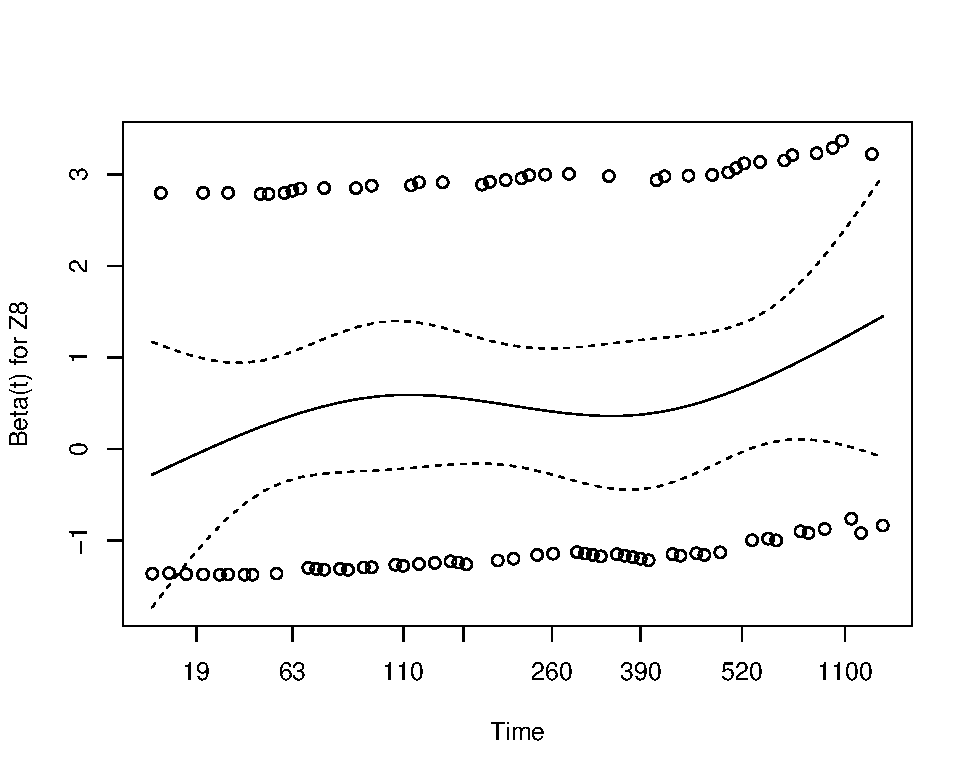
\includegraphics[width=0.8\linewidth]{Lista_5_files/figure-latex/unnamed-chunk-9-1} \end{center}

Em que se pode notar que a variável tratamento apresenta um
comportamento próximo de linear, não sendo possível traçar uma reta ao
longo do tempo.

Fazendo a tabela com o resultado do teste, em que:
\[ \left\{ \begin{array}{ll}
H_0: O \ modelo \ e \ de \ riscos \ proporcionais \\
H_1: O \ modelo \ nao \ e \ de \ riscos \ proporcionais  \end{array} \right.\ \]

\begin{longtable}[]{@{}lrrr@{}}
\toprule
& chisq & df & p\tabularnewline
\midrule
\endhead
Z8 & 1.591 & 1 & 0.207\tabularnewline
GLOBAL & 1.591 & 1 & 0.207\tabularnewline
\bottomrule
\end{longtable}

Queremos testar se o modelo de riscos proporcionais se adequa a esse
caso, e ao observar a tabela acima assim como resultado do gráfico acima
a variável tratamento não se rejeita a hipótese nula com um p-valor de
0.207 considerando um nível de significância de 5\%, ou seja, ela se
adequa no modelo de riscos proporcionais.

E com isso podemos concluir que as funções de sobrevivência para
indivíduos com a variável Z8 igual a 0 e igual a 1 são razoavelmente
paralelas ao longo de todo tempo. Ainda é possível dizer que indivíduos
que assumem o valor 1 para a variável Z8 possuem 1.649 vezes de ir a
óbito em relação a indivíduos que assumem o valor 0 para a variável Z8.

\newpage

\section{Exercício 2}\label{exercicio-2}

Um estudo foi conduzido para estudar se uma determinada droga era
cancerígena ou não. Para isso, foram selecionadas 50 ninhadas de ratos
e, de cada ninhada, foram selecionados 3 ratos. Dos ratos de cada
ninhada, selecionou-se aleatoriamente um deles para receber a droga e os
demais receberam placebo. Observou-se o tempo, em semanas, até o
desenvolvimento de um tumor. Os dados estão apresentados no arquivo
litter-data.csv.

\begin{enumerate}
\def\labelenumi{(\alph{enumi})}
\tightlist
\item
  Obtenha as curvas de Kaplan-Meier para os dois grupos e comente.
\end{enumerate}

\subsection{Resolução}\label{resolucao-3}

\begin{center}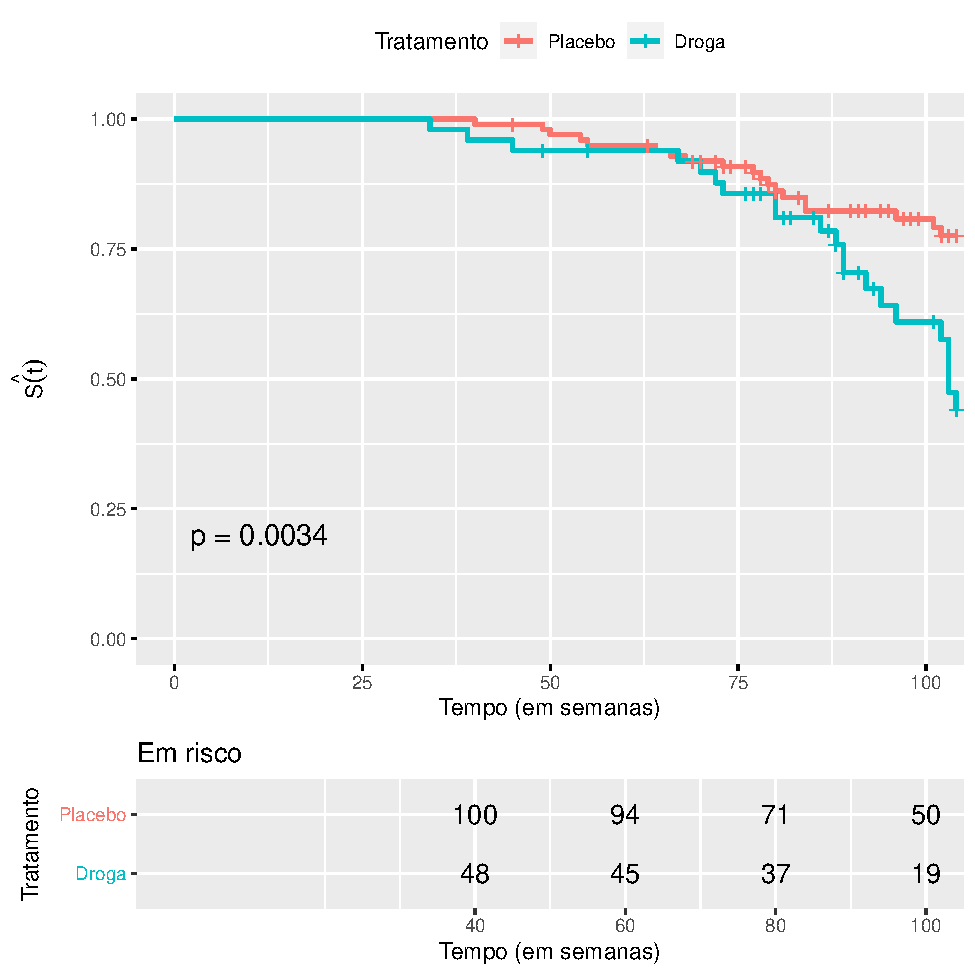
\includegraphics[width=0.8\linewidth]{Lista_5_files/figure-latex/unnamed-chunk-11-1} \end{center}

Em que podemos notar que as curvas são muito próximas com alguns
cruzamentos até o dia 88, depois disso há um distanciamento entre as
curvas a partir de então para os ratos que receberam a droga a curva
decresce mais rapidamente. Entretanto, nota-se muitas censuras para os
ratos que receberam placebo.

\begin{enumerate}
\def\labelenumi{(\alph{enumi})}
\setcounter{enumi}{1}
\tightlist
\item
  Ajuste um modelo de riscos proporcionais de Cox, ignorando o fato de
  existirem ratos pertencentes a uma mesma ninhada. Obtenha as
  estimativas dos parâmetros e interprete os resultados. Obtenha os
  resíduos de Schoenfeld para testar a proporcionalidade dos riscos.
  Faça um teste estatístico para a prpoporcionalidade dos riscos,
  utilizando a tranformação KM, ou seja, a curva de sobrevivência de
  Kaplan-Meier (versão contínua à esquerda).
\end{enumerate}

\subsection{Resolução}\label{resolucao-4}

Ajustando o modelo de riscos proporcionais de Cox, ignorando o fato de
existirem ratos pertencentes a uma mesma ninhadam, temos:

\begin{verbatim}
## Call:
## coxph(formula = Surv(Tempo, Delta) ~ Tratamento, data = litter_Data)
## 
##   n= 150, number of events= 40 
## 
##              coef exp(coef) se(coef)     z Pr(>|z|)   
## Tratamento 0.9047    2.4711   0.3175 2.849  0.00438 **
## ---
## Signif. codes:  0 '***' 0.001 '**' 0.01 '*' 0.05 '.' 0.1 ' ' 1
## 
##            exp(coef) exp(-coef) lower .95 upper .95
## Tratamento     2.471     0.4047     1.326     4.604
## 
## Concordance= 0.586  (se = 0.041 )
## Likelihood ratio test= 7.97  on 1 df,   p=0.005
## Wald test            = 8.12  on 1 df,   p=0.004
## Score (logrank) test = 8.68  on 1 df,   p=0.003
\end{verbatim}

Como temos um único parâmetro \(\beta\) a partir do modelo ajustado,
pode-se dizer que a taxa de ocorrência de tumores em ratos que recebem a
droga é 2.4 vezes a taxa associada a ratos que recebem placebo.

Resísudos de Schoenfeld com a tranformação KM:

\begin{center}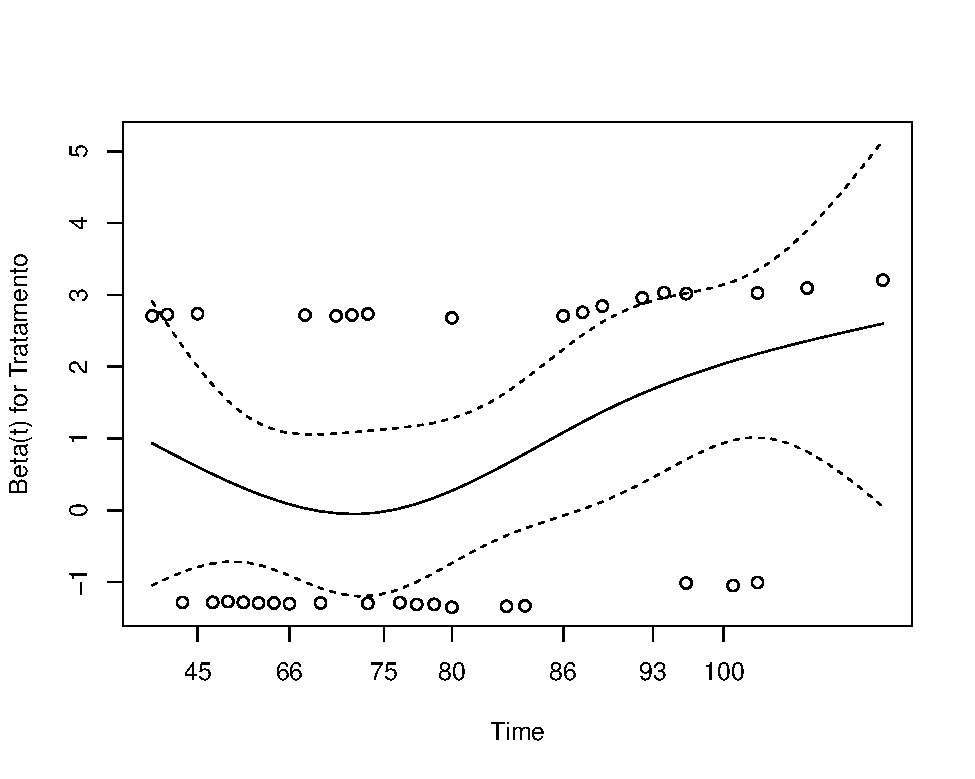
\includegraphics[width=0.8\linewidth]{Lista_5_files/figure-latex/unnamed-chunk-13-1} \end{center}

Em que se pode notar que a variável tratamento não apresenta um
comportamento linear, não sendo possível traçar uma reta ao longo do
tempo.

Fazendo a tabela com o resultado do teste, em que:
\[ \left\{ \begin{array}{ll}
H_0: O \ modelo \ e \ de \ riscos \ proporcionais \\
H_1: O \ modelo \ nao \ e \ de \ riscos \ proporcionais  \end{array} \right.\ \]

\begin{longtable}[]{@{}lrrr@{}}
\toprule
& chisq & df & p\tabularnewline
\midrule
\endhead
Tratamento & 5.02 & 1 & 0.025\tabularnewline
GLOBAL & 5.02 & 1 & 0.025\tabularnewline
\bottomrule
\end{longtable}

Queremos testar se o modelo de riscos proporcionais se adequa a esse
caso, e ao observar a tabela acima assim como resultado do gráfico acima
a variável tratamento rejeita a hipótese nula com um p-valor de 0.025
considerando um nível de significância de 5\%, ou seja, ela não se
adequa no modelo de riscos proporcionais.

\begin{enumerate}
\def\labelenumi{(\alph{enumi})}
\setcounter{enumi}{2}
\tightlist
\item
  Ajuste um modelo estratificado por ninhada, obtenha as estimativas e
  interprete os parâmetros. Obtenha os resíduos de Schoenfeld e faça o
  mesmo teste do item anterior para testar a proporcionalidade dos
  riscos. Compare os resultados.
\end{enumerate}

\subsection{Resolução}\label{resolucao-5}

Ajustando um modelo estratificado por ninhada, temos:

\begin{verbatim}
## Call:
## coxph(formula = Surv(Tempo, Delta) ~ Tratamento + strata(Ninhada), 
##     data = litter_Data)
## 
##   n= 150, number of events= 40 
## 
##              coef exp(coef) se(coef)     z Pr(>|z|)  
## Tratamento 0.8800    2.4110   0.3772 2.333   0.0196 *
## ---
## Signif. codes:  0 '***' 0.001 '**' 0.01 '*' 0.05 '.' 0.1 ' ' 1
## 
##            exp(coef) exp(-coef) lower .95 upper .95
## Tratamento     2.411     0.4148     1.151      5.05
## 
## Concordance= 0.67  (se = 0.088 )
## Likelihood ratio test= 5.58  on 1 df,   p=0.02
## Wald test            = 5.44  on 1 df,   p=0.02
## Score (logrank) test = 5.78  on 1 df,   p=0.02
\end{verbatim}

Como temos um único parâmetro \(\beta\) a partir do modelo ajustado,
pode-se dizer que a taxa de ocorrência de tumores em ratos que recebem a
droga é 2.5 vezes a taxa associada a ratos que recebem placebo.

Resísudos de Schoenfeld com a tranformação KM:

\begin{center}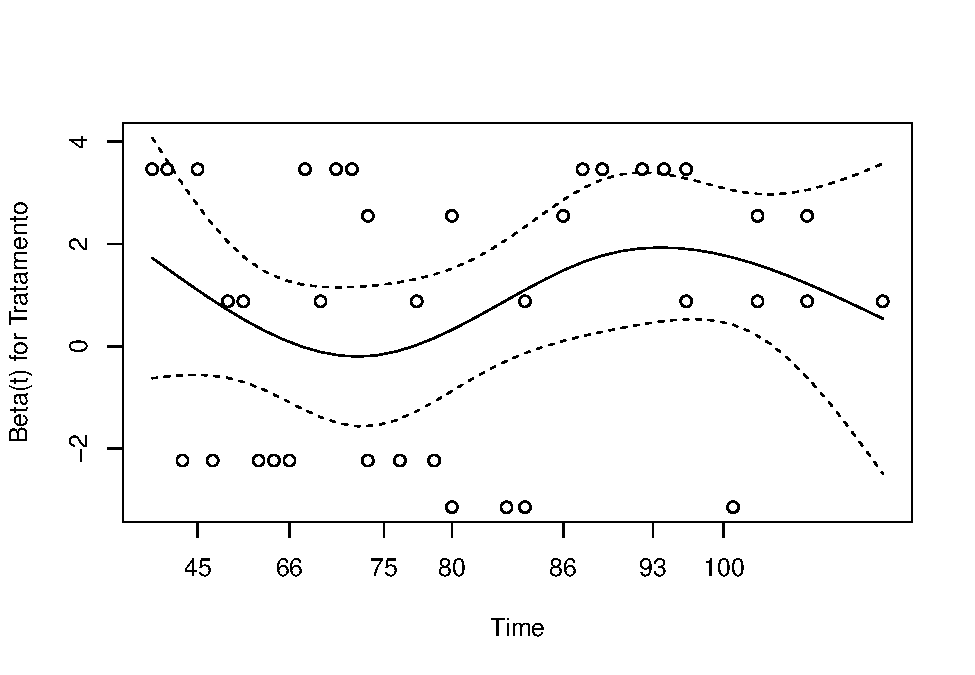
\includegraphics[width=0.8\linewidth]{Lista_5_files/figure-latex/unnamed-chunk-16-1} \end{center}

Em que se pode notar que a variável tratamento apresenta um
comportamento linear, sendo possível traçar uma reta ao longo do tempo.

Fazendo a tabela com o resultado do teste, em que:
\[ \left\{ \begin{array}{ll}
H_0: O \ modelo \ e \ de \ riscos \ proporcionais \\
H_1: O \ modelo \ nao \ e \ de \ riscos \ proporcionais  \end{array} \right.\ \]

\begin{longtable}[]{@{}lrrr@{}}
\toprule
& chisq & df & p\tabularnewline
\midrule
\endhead
Tratamento & 1.054 & 1 & 0.305\tabularnewline
GLOBAL & 1.054 & 1 & 0.305\tabularnewline
\bottomrule
\end{longtable}

Queremos testar se o modelo de riscos proporcionais se adequa a esse
caso, e ao observar a tabela acima assim como resultado do gráfico acima
a variável tratamento não se rejeita a hipótese nula com um p-valor de
0.305 considerando um nível de significância de 5\%, ou seja, ela se
adequa no modelo de riscos proporcionais.

Assim comparando com o item anterior, adicionando o efeito de ninhada,
assim como esperado a suposição de riscos proporcionais é satisfeita.

\section{Exercício 3}\label{exercicio-3}

Um estudo foi feito sobre o efeito da radiação na sobrevida de ratos. Um
grupo de ratos recebeu uma dose de 300 rad de radiação quando tinham
entre 5 e 6 semanas de vida e foram acompanhados até o óbito. Quando
morriam, os ratos eram necropsiados e a causa da morte determinada. Em
particular, os pesquisadores tinham interesse em estudar as mortes por
um tipo específico de linfoma um tipo de sarcoma.

Os tempos de vida, em dias, dos ratos e as causas das mortes estão
apresentadas na tabela abaixo.

\center

\begin{tabular}{lc}
\hline
\textbf{Causa da morte} & \textbf{Idade ao morrer (dias)} \\ \hline
Linfoma tímico & \begin{tabular}[c]{@{}c@{}}158, 192, 194, 195, 202, 215, 212, 215, 229, 230, 237,\\  240, 244, 247, 259, 300, 301, 337, 415, 444, 485, 496,\\ 529, 537, 624, 707, 800\end{tabular} \\
Sarcoma de células reticulares & \begin{tabular}[c]{@{}c@{}}430, 590, 606, 638, 655, 679, 691, 693, 696,\\ 747, 752, 760, 778, 821, 986\end{tabular} \\
Outras causas & \begin{tabular}[c]{@{}c@{}}136, 246, 255, 376, 421, 565, 616, 617, 652, 655, 658,\\ 660, 662, 675, 681, 734, 736, 737, 757, 769, 777, 801,\\ 807, 825, 855, 857, 864, 868, 870, 873, 882, 895, 910,\\ 934, 942, 1015, 1019\end{tabular} \\ \hline
\end{tabular}

\justify

\begin{enumerate}
\def\labelenumi{(\alph{enumi})}
\tightlist
\item
  Obtenha as curvas de incidência acumulada dos três riscos
  competitivos. Comente.
\end{enumerate}

\subsection{Resolução}\label{resolucao-6}

As curvas de incidência acumulada dos três riscos competitivos são:

\begin{center}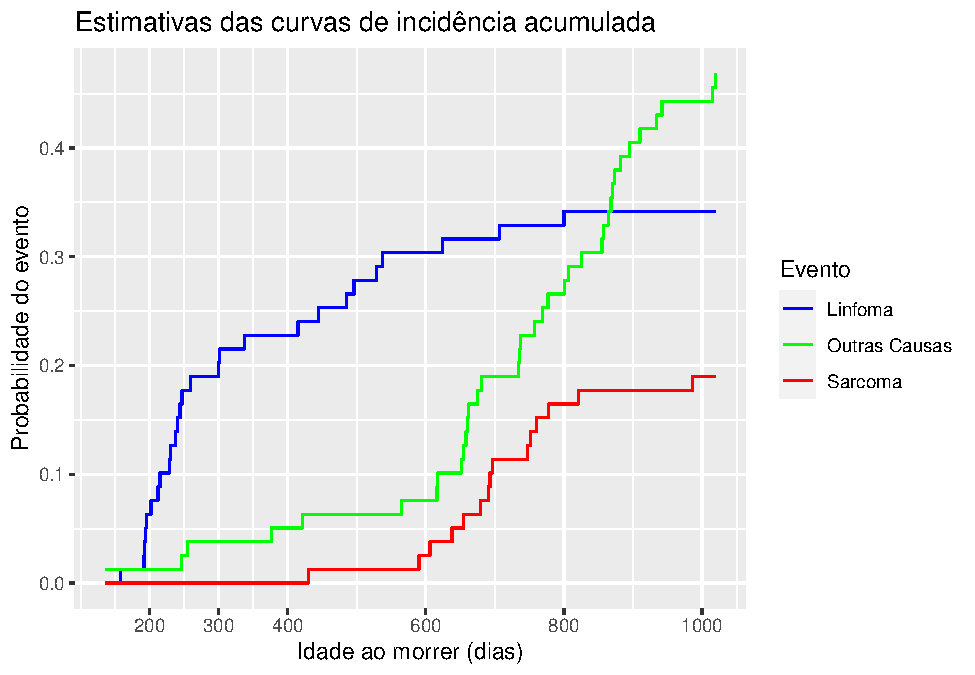
\includegraphics[width=0.8\linewidth]{Lista_5_files/figure-latex/unnamed-chunk-18-1} \end{center}

No gráfico acima apresentam-se as curvas referentes as estimativas de
probabilidade de falha por cada uma dos desfechos (competitivos entre
si) ao longo do tempo. Assim podemos observar que há um maior risco do
rato vir a sofrer primeiro uma morte por linfoma tímico, sendo seguido
por outras causas e com menor risco sarcoma de células reticulares atá
800 dias. No final do estudo há uma inversão das curvas, logo há um
maior risco do rato vir a sofrer primeiro uma morte por outras causas do
que por linfoma tímico.

\begin{enumerate}
\def\labelenumi{(\alph{enumi})}
\setcounter{enumi}{1}
\tightlist
\item
  Obtenha os valores estimados das funções de incidência acumulada dos
  três riscos competitivos nos instantes t = 200, 300, 400, 600, 800 e
  1000.
\end{enumerate}

\subsection{Resolução}\label{resolucao-7}

Os valores estimados das funções de incidência acumulada dos três riscos
competitivos nos instantes t = 200, 300, 400, 600, 800 e 1000 são:

\begin{longtable}[]{@{}rrrr@{}}
\toprule
time & Linfoma & Outras Causas & Sarcoma\tabularnewline
\midrule
\endhead
200 & 0.063 & 0.013 & 0.000\tabularnewline
300 & 0.203 & 0.038 & 0.000\tabularnewline
400 & 0.228 & 0.051 & 0.000\tabularnewline
600 & 0.304 & 0.076 & 0.025\tabularnewline
800 & 0.342 & 0.266 & 0.165\tabularnewline
1000 & 0.342 & 0.443 & 0.190\tabularnewline
\bottomrule
\end{longtable}

\begin{enumerate}
\def\labelenumi{(\alph{enumi})}
\setcounter{enumi}{2}
\tightlist
\item
  Obtenha a curva de Kaplan Meier da sobrevivência global dos dados.
  Calcule o valor da função de sobrevivência nos instantes t = 200, 300,
  400, 600, 800 e 1000. Observe que a soma dos valores das funções do
  incidência acumulada em cada instante é igual a 1 menos o valor da
  curva de Kaplan-Meier naquele ponto.
\end{enumerate}

\subsection{Resolução}\label{resolucao-8}

A curva de Kaplan Meier da sobrevivência global dos dados:

\begin{center}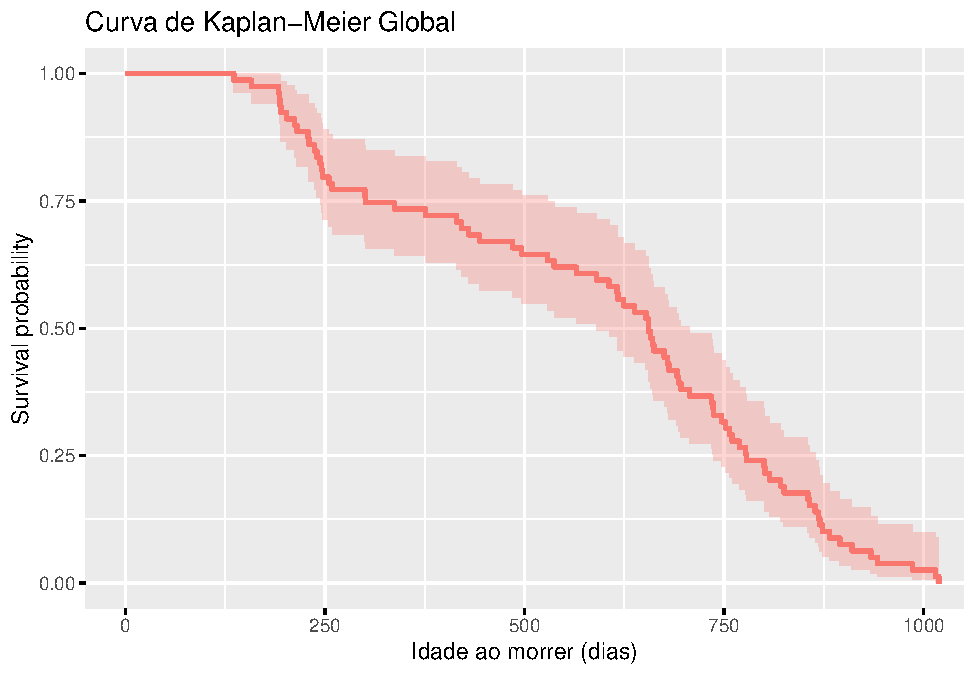
\includegraphics[width=0.8\linewidth]{Lista_5_files/figure-latex/unnamed-chunk-20-1} \end{center}

E os valores da função de sobrevivência nos instantes t = 200, 300, 400,
600, 800 e 1000 são:

\begin{longtable}[]{@{}rrr@{}}
\toprule
time & km & 1-km\tabularnewline
\midrule
\endhead
200 & 0.924 & 0.076\tabularnewline
300 & 0.759 & 0.241\tabularnewline
400 & 0.722 & 0.278\tabularnewline
600 & 0.595 & 0.405\tabularnewline
800 & 0.228 & 0.772\tabularnewline
1000 & 0.025 & 0.975\tabularnewline
\bottomrule
\end{longtable}

Em que podemos observar que a soma dos valores das funções do incidência
acumulada em cada instante é igual a 1 menos o valor da curva de
Kaplan-Meier naquele ponto.

\begin{enumerate}
\def\labelenumi{(\alph{enumi})}
\setcounter{enumi}{3}
\tightlist
\item
  Obtenha as curvas de sobrevivência de Kaplan Meier marginal dos dados,
  para cada tipo de evento, considerando a ocorrência dos outros eventos
  como censuras à direita. Coloque em um mesmo gráfico as curvas de
  inciência acumulada e 1 menos a curva de Kaplan-Meier.
\end{enumerate}

Compare e comente as diferenças, enfatizando o que cada curva de fato
estima.

\subsection{Resolução}\label{resolucao-9}

As curvas de sobrevivência de Kaplan Meier marginal dos dados, para cada
tipo de evento, considerando a ocorrência dos outros eventos como
censuras à direita:

\begin{center}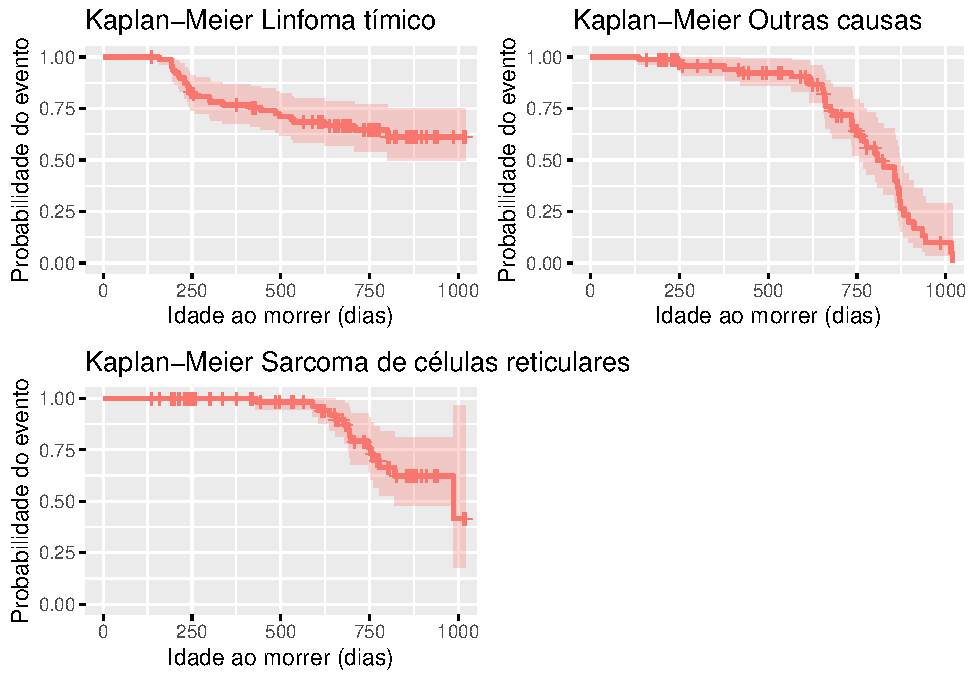
\includegraphics[width=0.8\linewidth]{Lista_5_files/figure-latex/unnamed-chunk-22-1} \end{center}

Em que se pode notar que a curva por linfoma tímico decai mais
suavemente a partir de 200 dias, a curva por outras causas, por sua vez,
decai mais rapidamente a partir de 600 dias e a curva por sarcoma de
células reticulares decai de forma suave a partir de 600 dias de estudo.

E as curvas de incidencia acumulada e de 1-km, temos:

\begin{center}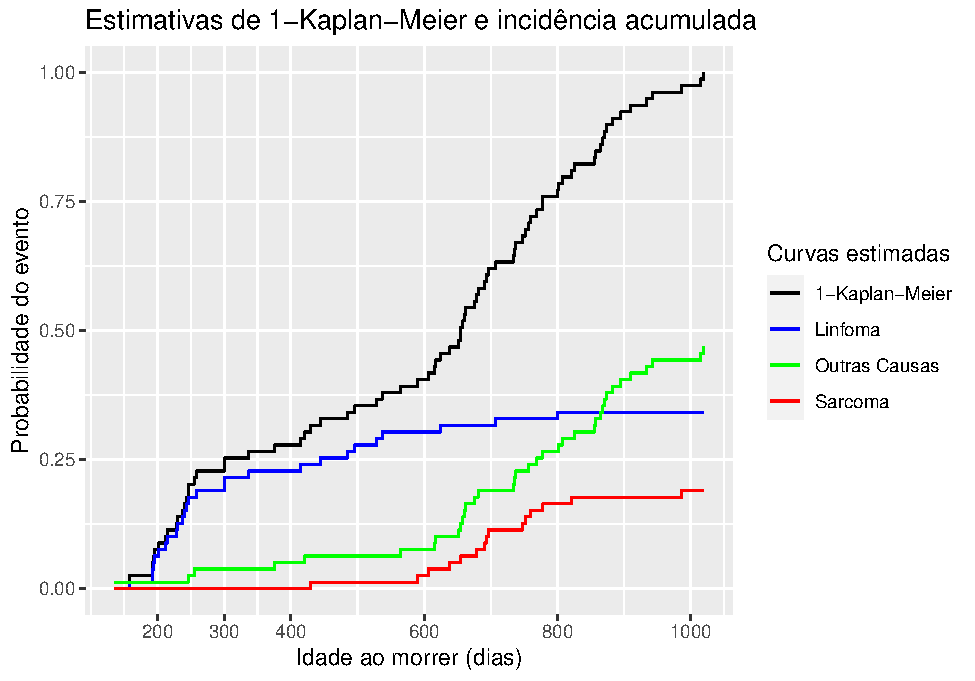
\includegraphics[width=0.8\linewidth]{Lista_5_files/figure-latex/unnamed-chunk-23-1} \end{center}

Nota-se que a curva 1-Kaplan-Meier seria a soma das curvas azul, verde e
vermelha, ou seja a probabilidade de qualquer um dos 3 eventos ocorrer.

\section{Códigos}\label{codigos}

\begin{Shaded}
\begin{Highlighting}[]
\CommentTok{# local de trabalho }
\KeywordTok{setwd}\NormalTok{(}\StringTok{"~/Área de Trabalho/Lista 5"}\NormalTok{)}

\CommentTok{# Pacotes}
\KeywordTok{library}\NormalTok{(ggplot2)}
\KeywordTok{library}\NormalTok{(survival)}
\KeywordTok{library}\NormalTok{(survminer)}
\KeywordTok{library}\NormalTok{(KMsurv)}
\KeywordTok{library}\NormalTok{(cmprsk)}
\KeywordTok{library}\NormalTok{(readr)}

\CommentTok{# Exercício 1}

\CommentTok{# Dados}
\NormalTok{BMT_DataOBITO <-}\StringTok{ }\KeywordTok{read_delim}\NormalTok{(}\StringTok{"BMT_DataOBITO.csv"}\NormalTok{,}\StringTok{";"}\NormalTok{, }
                            \DataTypeTok{escape_double =} \OtherTok{FALSE}\NormalTok{, }\DataTypeTok{trim_ws =} \OtherTok{TRUE}\NormalTok{)}
\NormalTok{BMT_DataRELAPSED <-}\StringTok{ }\KeywordTok{read_delim}\NormalTok{(}\StringTok{"BMT_DataRELAPSED.csv"}\NormalTok{,}\StringTok{";"}\NormalTok{, }
                               \DataTypeTok{escape_double =} \OtherTok{FALSE}\NormalTok{, }\DataTypeTok{trim_ws =} \OtherTok{TRUE}\NormalTok{)}

\CommentTok{# item b}

\CommentTok{# modelo inicial}
\NormalTok{modelo1.cox <-}\StringTok{ }\KeywordTok{coxph}\NormalTok{(}\KeywordTok{Surv}\NormalTok{(Tinicio, Tfim, Delta2)}\OperatorTok{~}\NormalTok{A}\OperatorTok{+}\NormalTok{C}\OperatorTok{+}\NormalTok{Z1}\OperatorTok{+}\NormalTok{Z3}\OperatorTok{+}\NormalTok{Z7}\OperatorTok{+}\NormalTok{Z8}\OperatorTok{+}\NormalTok{Z10,}
                     \DataTypeTok{data=}\NormalTok{BMT_DataRELAPSED)}
\KeywordTok{summary}\NormalTok{(modelo1.cox)}

\NormalTok{knitr}\OperatorTok{::}\KeywordTok{kable}\NormalTok{(}\KeywordTok{drop1}\NormalTok{(modelo1.cox, }\DataTypeTok{test=}\StringTok{"Chisq"}\NormalTok{),}\DataTypeTok{digits =} \DecValTok{3}\NormalTok{)}

\CommentTok{# modelo final}
\NormalTok{modelo2.cox <-}\StringTok{ }\KeywordTok{coxph}\NormalTok{(}\KeywordTok{Surv}\NormalTok{(Tinicio, Tfim, Delta2)}\OperatorTok{~}\NormalTok{Z8, }\DataTypeTok{data=}\NormalTok{BMT_DataRELAPSED)}
\KeywordTok{summary}\NormalTok{(modelo2.cox)}

\KeywordTok{drop1}\NormalTok{(modelo2.cox, }\DataTypeTok{test=}\StringTok{"Chisq"}\NormalTok{)}

\CommentTok{# resíduos de Schoenfeld}
\NormalTok{zph <-}\StringTok{ }\KeywordTok{cox.zph}\NormalTok{(modelo2.cox)}
\KeywordTok{plot}\NormalTok{(zph)}
\NormalTok{knitr}\OperatorTok{::}\KeywordTok{kable}\NormalTok{(zph}\OperatorTok{$}\NormalTok{table,}\DataTypeTok{digits =} \DecValTok{3}\NormalTok{)}

\CommentTok{# item c}
\CommentTok{# modelo inicial}
\NormalTok{modelo3.cox <-}\StringTok{ }\KeywordTok{coxph}\NormalTok{(}\KeywordTok{Surv}\NormalTok{(Tinicio, Tfim, Delta1)}\OperatorTok{~}\NormalTok{.}\OperatorTok{-}\NormalTok{Id, }\DataTypeTok{data=}\NormalTok{BMT_DataOBITO)}
\KeywordTok{summary}\NormalTok{(modelo3.cox)}

\KeywordTok{drop1}\NormalTok{(modelo3.cox, }\DataTypeTok{test=}\StringTok{"Chisq"}\NormalTok{)}

\CommentTok{# modelo final}
\NormalTok{modelo4.cox <-}\StringTok{ }\KeywordTok{coxph}\NormalTok{(}\KeywordTok{Surv}\NormalTok{(Tinicio, Tfim, Delta1)}\OperatorTok{~}\NormalTok{Z8, }\DataTypeTok{data=}\NormalTok{BMT_DataOBITO)}
\KeywordTok{summary}\NormalTok{(modelo4.cox)}

\NormalTok{knitr}\OperatorTok{::}\KeywordTok{kable}\NormalTok{(}\KeywordTok{drop1}\NormalTok{(modelo3.cox, }\DataTypeTok{test=}\StringTok{"Chisq"}\NormalTok{),}\DataTypeTok{digits =} \DecValTok{3}\NormalTok{)}

\CommentTok{# resíduos de Schoenfeld}
\NormalTok{zph2 <-}\StringTok{ }\KeywordTok{cox.zph}\NormalTok{(modelo4.cox)}
\KeywordTok{plot}\NormalTok{(zph2)}
\NormalTok{knitr}\OperatorTok{::}\KeywordTok{kable}\NormalTok{(zph2}\OperatorTok{$}\NormalTok{table,}\DataTypeTok{digits =} \DecValTok{3}\NormalTok{)}

\CommentTok{# Exercício 2}

\CommentTok{# dados}
\NormalTok{litter_Data <-}\StringTok{ }\KeywordTok{read.csv}\NormalTok{(}\StringTok{"litter-data.csv"}\NormalTok{)}

\CommentTok{# Kaplan Meier}
\NormalTok{KM <-}\StringTok{ }\KeywordTok{survfit}\NormalTok{(}\KeywordTok{Surv}\NormalTok{(Tempo,Delta)}\OperatorTok{~}\StringTok{ }\NormalTok{Tratamento,}\DataTypeTok{data =}\NormalTok{ litter_Data)}

\CommentTok{# Grafico Kaplan-Meier}
\KeywordTok{ggsurvplot}\NormalTok{(KM, }\DataTypeTok{data =}\NormalTok{litter_Data, }\DataTypeTok{linetype =} \DecValTok{1}\NormalTok{,  }\DataTypeTok{risk.table =} \OtherTok{TRUE}\NormalTok{,}
           \DataTypeTok{xlab=}\StringTok{"Tempo (em semanas)"}\NormalTok{,}
           \DataTypeTok{ylab=}\KeywordTok{expression}\NormalTok{(}\KeywordTok{hat}\NormalTok{(}\KeywordTok{S}\NormalTok{(t))), }\DataTypeTok{risk.table.title=}\StringTok{"Em risco"}\NormalTok{,}
           \DataTypeTok{legend.title =}\StringTok{"Tratamento"}\NormalTok{,}\DataTypeTok{ggtheme=}\KeywordTok{theme_gray}\NormalTok{(),}
           \DataTypeTok{legend.labs=}\KeywordTok{c}\NormalTok{(}\StringTok{"Placebo"}\NormalTok{, }\StringTok{"Droga"}\NormalTok{), }\DataTypeTok{pval=}\OtherTok{TRUE}\NormalTok{)}

\CommentTok{# item b}

\CommentTok{# modelo de cox ignorando ninhada}
\NormalTok{cox_fit1 <-}\StringTok{ }\KeywordTok{coxph}\NormalTok{(}\KeywordTok{Surv}\NormalTok{(Tempo, Delta)}\OperatorTok{~}\StringTok{ }\NormalTok{Tratamento,}\DataTypeTok{data=}\NormalTok{litter_Data)}
\KeywordTok{summary}\NormalTok{(cox_fit1)}

\CommentTok{# Residuos de Schoenfeld}
\NormalTok{zph_km <-}\StringTok{ }\KeywordTok{cox.zph}\NormalTok{(cox_fit1,}\DataTypeTok{transform=}\StringTok{'km'}\NormalTok{)}

\KeywordTok{plot}\NormalTok{(zph_km)}

\CommentTok{# tabela do testeS}
\NormalTok{knitr}\OperatorTok{::}\KeywordTok{kable}\NormalTok{(zph_km}\OperatorTok{$}\NormalTok{table,}\DataTypeTok{digits =} \DecValTok{3}\NormalTok{)}

\CommentTok{# item c}

\CommentTok{# modelo de cox estratificado por ninhada}
\NormalTok{cox_strat_fit2 <-}\KeywordTok{coxph}\NormalTok{(}\KeywordTok{Surv}\NormalTok{(Tempo, Delta)}\OperatorTok{~}\StringTok{ }\NormalTok{Tratamento}\OperatorTok{+}\KeywordTok{strata}\NormalTok{(Ninhada),}
                       \DataTypeTok{data =}\NormalTok{ litter_Data)}
\KeywordTok{summary}\NormalTok{(cox_strat_fit2)}

\CommentTok{# Residuos de Schoenfeld}
\NormalTok{zph_km2 <-}\StringTok{ }\KeywordTok{cox.zph}\NormalTok{(cox_strat_fit2,}\DataTypeTok{transform=}\StringTok{'km'}\NormalTok{)}

\KeywordTok{plot}\NormalTok{(zph_km2)}

\CommentTok{# tabela do teste}
\NormalTok{knitr}\OperatorTok{::}\KeywordTok{kable}\NormalTok{(zph_km2}\OperatorTok{$}\NormalTok{table,}\DataTypeTok{digits =} \DecValTok{3}\NormalTok{)}

\CommentTok{# Exercício 3}

\CommentTok{# Dados}
\NormalTok{lin <-}\StringTok{ }\KeywordTok{c}\NormalTok{(}\DecValTok{158}\NormalTok{, }\DecValTok{192}\NormalTok{, }\DecValTok{193}\NormalTok{, }\DecValTok{194}\NormalTok{, }\DecValTok{195}\NormalTok{, }\DecValTok{202}\NormalTok{, }\DecValTok{212}\NormalTok{, }\DecValTok{215}\NormalTok{, }\DecValTok{229}\NormalTok{, }\DecValTok{230}\NormalTok{, }\DecValTok{237}\NormalTok{,}
         \DecValTok{240}\NormalTok{, }\DecValTok{244}\NormalTok{, }\DecValTok{247}\NormalTok{, }\DecValTok{259}\NormalTok{, }\DecValTok{300}\NormalTok{, }\DecValTok{301}\NormalTok{, }\DecValTok{337}\NormalTok{, }\DecValTok{415}\NormalTok{, }\DecValTok{444}\NormalTok{, }\DecValTok{485}\NormalTok{, }\DecValTok{496}\NormalTok{,}
         \DecValTok{529}\NormalTok{, }\DecValTok{537}\NormalTok{, }\DecValTok{624}\NormalTok{, }\DecValTok{707}\NormalTok{, }\DecValTok{800}\NormalTok{)}
\NormalTok{sar <-}\StringTok{  }\KeywordTok{c}\NormalTok{(}\DecValTok{430}\NormalTok{, }\DecValTok{590}\NormalTok{, }\DecValTok{606}\NormalTok{, }\DecValTok{638}\NormalTok{, }\DecValTok{655}\NormalTok{, }\DecValTok{679}\NormalTok{, }\DecValTok{691}\NormalTok{, }\DecValTok{693}\NormalTok{, }\DecValTok{696}\NormalTok{,}
          \DecValTok{747}\NormalTok{, }\DecValTok{752}\NormalTok{, }\DecValTok{760}\NormalTok{, }\DecValTok{778}\NormalTok{, }\DecValTok{821}\NormalTok{, }\DecValTok{986}\NormalTok{)}
\NormalTok{out <-}\StringTok{ }\KeywordTok{c}\NormalTok{(}\DecValTok{136}\NormalTok{, }\DecValTok{246}\NormalTok{, }\DecValTok{255}\NormalTok{, }\DecValTok{376}\NormalTok{, }\DecValTok{421}\NormalTok{, }\DecValTok{565}\NormalTok{, }\DecValTok{616}\NormalTok{, }\DecValTok{617}\NormalTok{, }\DecValTok{652}\NormalTok{, }\DecValTok{655}\NormalTok{, }\DecValTok{658}\NormalTok{,}
         \DecValTok{660}\NormalTok{, }\DecValTok{662}\NormalTok{, }\DecValTok{675}\NormalTok{, }\DecValTok{681}\NormalTok{, }\DecValTok{734}\NormalTok{, }\DecValTok{736}\NormalTok{, }\DecValTok{737}\NormalTok{, }\DecValTok{757}\NormalTok{, }\DecValTok{769}\NormalTok{, }\DecValTok{777}\NormalTok{, }\DecValTok{801}\NormalTok{,}
         \DecValTok{807}\NormalTok{, }\DecValTok{825}\NormalTok{, }\DecValTok{855}\NormalTok{, }\DecValTok{857}\NormalTok{, }\DecValTok{864}\NormalTok{, }\DecValTok{868}\NormalTok{, }\DecValTok{870}\NormalTok{, }\DecValTok{873}\NormalTok{, }\DecValTok{882}\NormalTok{, }\DecValTok{895}\NormalTok{, }\DecValTok{910}\NormalTok{,}
         \DecValTok{934}\NormalTok{, }\DecValTok{942}\NormalTok{, }\DecValTok{1015}\NormalTok{, }\DecValTok{1019}\NormalTok{)}

\NormalTok{causa <-}\StringTok{ }\KeywordTok{factor}\NormalTok{(}\KeywordTok{c}\NormalTok{(}\KeywordTok{rep}\NormalTok{(}\StringTok{'Linfoma'}\NormalTok{,}\DecValTok{27}\NormalTok{),}\KeywordTok{rep}\NormalTok{(}\StringTok{'Sarcoma'}\NormalTok{,}\DecValTok{15}\NormalTok{),}\KeywordTok{rep}\NormalTok{(}\StringTok{'Outras_Causas'}\NormalTok{,}\DecValTok{37}\NormalTok{)))}
\NormalTok{tempo <-}\StringTok{ }\KeywordTok{c}\NormalTok{(lin,sar,out)}
\NormalTok{data3 <-}\StringTok{ }\KeywordTok{data.frame}\NormalTok{(tempo,causa)}

\CommentTok{# item a}

\CommentTok{# estimativas das curvas de incidência acumulada}
\NormalTok{CIF <-}\StringTok{ }\KeywordTok{cuminc}\NormalTok{(tempo,}\KeywordTok{factor}\NormalTok{(causa), }\DataTypeTok{cencode =} \DecValTok{0}\NormalTok{)}

\CommentTok{# Estimativas de km globais}
\NormalTok{KM3 <-}\StringTok{ }\KeywordTok{survfit}\NormalTok{(}\KeywordTok{Surv}\NormalTok{(tempo)}\OperatorTok{~}\DecValTok{1}\NormalTok{,}\DataTypeTok{data =}\NormalTok{ data3)}

\CommentTok{# dados para 1-km e cuvras de incidência acumulada}
\NormalTok{df3d <-}\StringTok{ }\KeywordTok{data.frame}\NormalTok{(KM3}\OperatorTok{$}\NormalTok{time,}\DecValTok{1}\OperatorTok{-}\NormalTok{KM3}\OperatorTok{$}\NormalTok{surv,}
                   \KeywordTok{t}\NormalTok{(}\KeywordTok{timepoints}\NormalTok{(CIF, }\DataTypeTok{times =}\NormalTok{ data3}\OperatorTok{$}\NormalTok{tempo)}\OperatorTok{$}\NormalTok{est))}

\KeywordTok{colnames}\NormalTok{(df3d) <-}\StringTok{ }\KeywordTok{c}\NormalTok{(}\StringTok{"time"}\NormalTok{,}\StringTok{"F"}\NormalTok{,}\StringTok{"Linfoma"}\NormalTok{,}\StringTok{"Outras_Causas"}\NormalTok{,}\StringTok{"Sarcoma"}\NormalTok{)}

\CommentTok{# cores}
\NormalTok{colors <-}\StringTok{ }\KeywordTok{c}\NormalTok{(}\StringTok{"Linfoma"}\NormalTok{ =}\StringTok{ "Blue"}\NormalTok{,}
            \StringTok{"Sarcoma"}\NormalTok{ =}\StringTok{ "Red"}\NormalTok{,}
            \StringTok{"Outras Causas"}\NormalTok{ =}\StringTok{ "Green"}\NormalTok{)}

\CommentTok{# curvas das estimativas das curvas de incidência acumulada}
\KeywordTok{ggplot}\NormalTok{(}\DataTypeTok{data =}\NormalTok{ df3d) }\OperatorTok{+}\StringTok{  }
\StringTok{  }\KeywordTok{geom_step}\NormalTok{(}\KeywordTok{aes}\NormalTok{(}\DataTypeTok{x =}\NormalTok{ time, }\DataTypeTok{y =}\NormalTok{ Linfoma,}\DataTypeTok{color =} \StringTok{"Linfoma"}\NormalTok{)) }\OperatorTok{+}
\StringTok{  }\KeywordTok{geom_step}\NormalTok{(}\KeywordTok{aes}\NormalTok{(}\DataTypeTok{x =}\NormalTok{ time, }\DataTypeTok{y =}\NormalTok{ Sarcoma,}\DataTypeTok{color =} \StringTok{"Sarcoma"}\NormalTok{)) }\OperatorTok{+}
\StringTok{  }\KeywordTok{geom_step}\NormalTok{(}\KeywordTok{aes}\NormalTok{(}\DataTypeTok{x =}\NormalTok{ time, }\DataTypeTok{y =}\NormalTok{ Outras_Causas,}\DataTypeTok{color =} \StringTok{"Outras Causas"}\NormalTok{)) }\OperatorTok{+}
\StringTok{  }\KeywordTok{scale_x_continuous}\NormalTok{(}\DataTypeTok{breaks =} \KeywordTok{c}\NormalTok{(}\DecValTok{200}\NormalTok{,}\DecValTok{300}\NormalTok{,}\DecValTok{400}\NormalTok{,}\DecValTok{600}\NormalTok{,}\DecValTok{800}\NormalTok{,}\DecValTok{1000}\NormalTok{)) }\OperatorTok{+}
\StringTok{  }\KeywordTok{scale_color_manual}\NormalTok{(}\DataTypeTok{values =}\NormalTok{ colors) }\OperatorTok{+}
\StringTok{  }\KeywordTok{labs}\NormalTok{(}\DataTypeTok{x=}\StringTok{"Idade ao morrer (dias)"}\NormalTok{,}
       \DataTypeTok{y=}\StringTok{"Probabilidade do evento"}\NormalTok{,}
       \DataTypeTok{title =} \StringTok{"Estimativas das curvas de incidência acumulada"}\NormalTok{,}
       \DataTypeTok{color =} \StringTok{"Evento"}\NormalTok{) }

\CommentTok{# item b}
\NormalTok{knitr}\OperatorTok{::}\KeywordTok{kable}\NormalTok{(}\KeywordTok{data.frame}\NormalTok{(}\DataTypeTok{time =} \KeywordTok{c}\NormalTok{(}\DecValTok{200}\NormalTok{,}\DecValTok{300}\NormalTok{,}\DecValTok{400}\NormalTok{,}\DecValTok{600}\NormalTok{,}\DecValTok{800}\NormalTok{,}\DecValTok{1000}\NormalTok{),}
  \KeywordTok{t}\NormalTok{(}\KeywordTok{timepoints}\NormalTok{(CIF, }\DataTypeTok{times =} \KeywordTok{c}\NormalTok{(}\DecValTok{200}\NormalTok{,}\DecValTok{300}\NormalTok{,}\DecValTok{400}\NormalTok{,}\DecValTok{600}\NormalTok{,}\DecValTok{800}\NormalTok{,}\DecValTok{1000}\NormalTok{))}\OperatorTok{$}\NormalTok{est)),}
  \DataTypeTok{digits =} \DecValTok{3}\NormalTok{,}\DataTypeTok{row.names =}\NormalTok{ F,}\DataTypeTok{col.names =} \KeywordTok{c}\NormalTok{(}\StringTok{"time"}\NormalTok{,}\StringTok{"Linfoma"}\NormalTok{,}\StringTok{"Outras Causas"}\NormalTok{,}\StringTok{"Sarcoma"}\NormalTok{))}

\CommentTok{# item c}

\CommentTok{# Grafico Kaplan-Meier global}
\KeywordTok{ggsurvplot}\NormalTok{(KM3, }\DataTypeTok{data =}\NormalTok{ data3, }\DataTypeTok{linetype =} \DecValTok{1}\NormalTok{, }\DataTypeTok{xlab=}\StringTok{"Idade ao morrer (dias)"}\NormalTok{,}\DataTypeTok{legend=}\StringTok{'none'}\NormalTok{,}
           \DataTypeTok{title=}\StringTok{'Curva de Kaplan-Meier Global'}\NormalTok{,}
           \DataTypeTok{ggtheme=}\KeywordTok{theme_gray}\NormalTok{())}

\CommentTok{# tabela com as estimavivas de km para o t=200,300,400,600,800 e 1000}
\NormalTok{table <-}\StringTok{ }\KeywordTok{summary}\NormalTok{(KM3,}\DataTypeTok{time=}\KeywordTok{c}\NormalTok{(}\DecValTok{200}\NormalTok{,}\DecValTok{300}\NormalTok{,}\DecValTok{400}\NormalTok{,}\DecValTok{600}\NormalTok{,}\DecValTok{800}\NormalTok{,}\DecValTok{1000}\NormalTok{))}
\NormalTok{table <-}\StringTok{ }\KeywordTok{data.frame}\NormalTok{(table}\OperatorTok{$}\NormalTok{time,table}\OperatorTok{$}\NormalTok{surv,}\DecValTok{1}\OperatorTok{-}\NormalTok{table}\OperatorTok{$}\NormalTok{surv)}
\KeywordTok{colnames}\NormalTok{(table) <-}\StringTok{ }\KeywordTok{c}\NormalTok{(}\StringTok{"time"}\NormalTok{, }\StringTok{"km"}\NormalTok{,}\StringTok{"1-km"}\NormalTok{)}
\NormalTok{knitr}\OperatorTok{::}\KeywordTok{kable}\NormalTok{(table,}\DataTypeTok{digits =} \DecValTok{3}\NormalTok{)}

\CommentTok{# item d}
\NormalTok{linf <-}\StringTok{ }\KeywordTok{ifelse}\NormalTok{(causa}\OperatorTok{==}\StringTok{'Linfoma'}\NormalTok{,}\DecValTok{1}\NormalTok{,}\DecValTok{0}\NormalTok{)}
\NormalTok{sarc <-}\StringTok{ }\KeywordTok{ifelse}\NormalTok{(causa}\OperatorTok{==}\StringTok{'Sarcoma'}\NormalTok{,}\DecValTok{1}\NormalTok{,}\DecValTok{0}\NormalTok{)}
\NormalTok{oc <-}\StringTok{ }\KeywordTok{ifelse}\NormalTok{(causa}\OperatorTok{==}\StringTok{'Outras_Causas'}\NormalTok{,}\DecValTok{1}\NormalTok{,}\DecValTok{0}\NormalTok{)}

\CommentTok{# Km evento linfoma}
\NormalTok{KM4 <-}\StringTok{ }\KeywordTok{survfit}\NormalTok{(}\KeywordTok{Surv}\NormalTok{(tempo,linf)}\OperatorTok{~}\DecValTok{1}\NormalTok{,}\DataTypeTok{data =}\NormalTok{ data3)}

\CommentTok{# Grafico Kaplan-Meier linfoma}
\NormalTok{plot1 <-}\StringTok{ }\KeywordTok{ggsurvplot}\NormalTok{(KM4,}\DataTypeTok{legend=}\StringTok{'none'}\NormalTok{,}
                    \DataTypeTok{title=}\StringTok{'Kaplan-Meier Linfoma tímico'}\NormalTok{,}
                    \DataTypeTok{ggtheme=}\KeywordTok{theme_gray}\NormalTok{()) }\OperatorTok{+}
\StringTok{                    }\KeywordTok{labs}\NormalTok{(}\DataTypeTok{y=}\StringTok{'Probabilidade do evento'}\NormalTok{,}
                         \DataTypeTok{x=}\StringTok{'Idade ao morrer (dias)'}\NormalTok{)}

\CommentTok{# Km evento sarcoma}
\NormalTok{KM5 <-}\StringTok{ }\KeywordTok{survfit}\NormalTok{(}\KeywordTok{Surv}\NormalTok{(tempo,sarc)}\OperatorTok{~}\DecValTok{1}\NormalTok{,}\DataTypeTok{data =}\NormalTok{ data3)}

\CommentTok{# Grafico Kaplan-Meier sarcoma}
\NormalTok{plot2 <-}\StringTok{ }\KeywordTok{ggsurvplot}\NormalTok{(KM5, }\DataTypeTok{legend=}\StringTok{'none'}\NormalTok{,}
                    \DataTypeTok{title=}\StringTok{'Kaplan-Meier Sarcoma de células reticulares'}\NormalTok{,}
                    \DataTypeTok{ggtheme=}\KeywordTok{theme_gray}\NormalTok{()) }\OperatorTok{+}
\StringTok{                    }\KeywordTok{labs}\NormalTok{(}\DataTypeTok{y=}\StringTok{'Probabilidade do evento'}\NormalTok{,}
                         \DataTypeTok{x=}\StringTok{'Idade ao morrer (dias)'}\NormalTok{)}

\CommentTok{# Km evento outras causas}
\NormalTok{KM6 <-}\StringTok{ }\KeywordTok{survfit}\NormalTok{(}\KeywordTok{Surv}\NormalTok{(tempo,oc)}\OperatorTok{~}\DecValTok{1}\NormalTok{,}\DataTypeTok{data =}\NormalTok{ data3)}

\CommentTok{# Grafico Kaplan-Meier outras causas}
\NormalTok{plot3 <-}\StringTok{ }\KeywordTok{ggsurvplot}\NormalTok{(KM6,}\DataTypeTok{legend=}\StringTok{'none'}\NormalTok{, }
                    \DataTypeTok{title=}\StringTok{'Kaplan-Meier Outras causas'}\NormalTok{,}
                    \DataTypeTok{ggtheme=}\KeywordTok{theme_gray}\NormalTok{()) }\OperatorTok{+}\StringTok{ }
\StringTok{                    }\KeywordTok{labs}\NormalTok{(}\DataTypeTok{y=}\StringTok{'Probabilidade do evento'}\NormalTok{,}
                         \DataTypeTok{x=}\StringTok{'Idade ao morrer (dias)'}\NormalTok{)}

\CommentTok{# PLot das 3 curvas}
\KeywordTok{arrange_ggsurvplots}\NormalTok{(}\KeywordTok{list}\NormalTok{(plot1, plot2, plot3), }
                    \DataTypeTok{print =} \OtherTok{TRUE}\NormalTok{,}\DataTypeTok{ncol =} \DecValTok{2}\NormalTok{, }\DataTypeTok{nrow =} \DecValTok{2}\NormalTok{)}

\CommentTok{# cores}
\NormalTok{colors <-}\StringTok{ }\KeywordTok{c}\NormalTok{(}\StringTok{"1-Kaplan-Meier"}\NormalTok{ =}\StringTok{ "Black"}\NormalTok{,}
            \StringTok{"Linfoma"}\NormalTok{ =}\StringTok{ "Blue"}\NormalTok{,}
            \StringTok{"Sarcoma"}\NormalTok{ =}\StringTok{ "Red"}\NormalTok{,}
            \StringTok{"Outras Causas"}\NormalTok{ =}\StringTok{ "Green"}\NormalTok{)}

\CommentTok{# Gráficos das estimativas de 1-Kaplan-Meier e incidência acumulada}
\KeywordTok{ggplot}\NormalTok{(}\DataTypeTok{data =}\NormalTok{ df3d) }\OperatorTok{+}\StringTok{  }
\StringTok{  }\KeywordTok{geom_step}\NormalTok{(}\KeywordTok{aes}\NormalTok{(}\DataTypeTok{x =}\NormalTok{ time, }\DataTypeTok{y =}\NormalTok{ F,}\DataTypeTok{color =} \StringTok{"1-Kaplan-Meier"}\NormalTok{)) }\OperatorTok{+}
\StringTok{  }\KeywordTok{geom_step}\NormalTok{(}\KeywordTok{aes}\NormalTok{(}\DataTypeTok{x =}\NormalTok{ time, }\DataTypeTok{y =}\NormalTok{ Linfoma,}\DataTypeTok{color =} \StringTok{"Linfoma"}\NormalTok{)) }\OperatorTok{+}
\StringTok{  }\KeywordTok{geom_step}\NormalTok{(}\KeywordTok{aes}\NormalTok{(}\DataTypeTok{x =}\NormalTok{ time, }\DataTypeTok{y =}\NormalTok{ Sarcoma,}\DataTypeTok{color =} \StringTok{"Sarcoma"}\NormalTok{)) }\OperatorTok{+}
\StringTok{  }\KeywordTok{geom_step}\NormalTok{(}\KeywordTok{aes}\NormalTok{(}\DataTypeTok{x =}\NormalTok{ time, }\DataTypeTok{y =}\NormalTok{ Outras_Causas,}\DataTypeTok{color =} \StringTok{"Outras Causas"}\NormalTok{)) }\OperatorTok{+}
\StringTok{  }\KeywordTok{scale_x_continuous}\NormalTok{(}\DataTypeTok{breaks =} \KeywordTok{c}\NormalTok{(}\DecValTok{200}\NormalTok{,}\DecValTok{300}\NormalTok{,}\DecValTok{400}\NormalTok{,}\DecValTok{600}\NormalTok{,}\DecValTok{800}\NormalTok{,}\DecValTok{1000}\NormalTok{)) }\OperatorTok{+}
\StringTok{  }\KeywordTok{scale_color_manual}\NormalTok{(}\DataTypeTok{values =}\NormalTok{ colors) }\OperatorTok{+}
\StringTok{  }\KeywordTok{labs}\NormalTok{(}\DataTypeTok{x=}\StringTok{"Idade ao morrer (dias)"}\NormalTok{,}
       \DataTypeTok{y=}\StringTok{"Probabilidade do evento"}\NormalTok{,}
       \DataTypeTok{title =} \StringTok{"Estimativas de 1-Kaplan-Meier e incidência acumulada"}\NormalTok{,}
       \DataTypeTok{color =} \StringTok{"Curvas estimadas"}\NormalTok{) }
\end{Highlighting}
\end{Shaded}


\end{document}
